\section{Nonlinear signal Analysis}

\subsection{Heart rate variability}
Heart is a pump which is synchronously activated by muscle contraction. The muscle motion is driven via the propagation of electrical potential. The heart beating manifests externally as changing potential in the body. The potential generated by beating heart dominates other electrical potential. Electrocardiography ECG measures this change in vector potential with multiple pairs of electrodes and a differential amplifier. The very standard measurement setup consist of 5 different electrodes into different parts of the body in figure \ref{icon3}. The wave front time-course in figure \ref{icon4} encodes the distinct phases of a heart beat. Whereby RR interval rate (tachogram) could be computed by measuring the distance in consecutive RR and the outcome. Algorithms for performing this computation are numerous where the most widely cited is Pan-Tompkins \cite{19} which is also outlined in \ref{algo1}. 

Tachogram is then utilized as an input signal for frameworks. Linear and nonlinear analysis are employed to detect irregular cardiac cycles via heart rate variability (HRV) analysis. HRV consistently reflects many physiological events, as a result it modulate the rhythmicity of a heart. It shows how heart respond when unpredictable stimuli reveals. HR signal has a non-stationary nature, wherein its variation could tell warnings about cardiac diseases. HRV possesses the ability to provide and overall estimate of the cardiac health as well as the autonomic nervous system \cite{20}. Moreover there are clear correlation of HRV and blood pressure, myocardial infarction, nervous system, cardiac arrhythmia, diabetes, renal failure, gender, age, drugs, smoking, alcohol and sleeping. Thereby, there are many evidences inferring that significant nonlinear contribution into the fluctuation of HR exists. 

Consequently, nonlinear approaches could better analyse the HR. Linear methods could actually assess the magnitude of the variability, however, there is still lack of ability to describe the dynamical properties of the fluctuations. Non-linearity arises due to highly dependency on small disturbances, the non-stationary nature of the signal and multiscale attitude of the time-course signal. Via nonlinear methods, on the other hand, it is possible to estimate the quality, scaling, correlation properties of the nonlinear characteristics of cardiovascular dynamics: It brings closer to the reality the understanding of irregularities event. Nevertheless, yet is not possible to precisely quantify the contribution of nonlinear indices. Additionally not comprehensive conclusion could be made for the nonlinear parameters from the physiological prospective. 




\subsection{Non-linear signal processing}

Tachogram can be described as a time series where its variables (RR intervals) are measured as a function of time. They don't have a steady state, that means there is no constant solution of a mathematical equation which can describe them all. This can be seen as a superposition of oscillation (heart beat) and irregular activities, namely, two distinct mathematical description: noise and chaos. Noise differently from chaos cannot be linked with any underlying or periodic process, whereas chaos arises in a deterministic system not necessarily from influence of external noise. Additionally, chaos is irregular but not a random event. It could be described by deterministic equation and at the same time not being predictable. It has a very sensitive dependency on initial conditions and may give rise to invariant sets with complex (fractal) boundaries.   

Tachogram on itself possesses a lot of similarity at all scales of observation, also known as self-similarity. Consequently, it could also be seen from the fractal prospective. Fractal is described as a pattern yet not differentiable and auto-correlated over a range of scales. Fractal dimension D is categorised via power-law relation, however, differently from Euclidean counterparts, they occupy more space. A curve of one dimension has a dimension of $1<D<2$ which is more than the Euclidean space. Fractal dimension D increases with surface roughness. 


Nonlinear HRV analysis is divided into two main categories. Scaling behavior of nonlinear systems could be quantified via:
\begin{itemize}
    \item Fractal dimension allows to measure the degree of complexity by evaluating how fast our measurement increases or decrease as our scale becomes larger or smaller. This fractal could rise due to chaos dynamics and one of the method for estimation of the dimension is box counting technique. 
    \item 1/f slope quantity is bounded between the white noise where there is no correlation in time and random walk noise with no correlation between increments. Fluctuation of heartbeat period has a power spectral density which behaves inversely proportional to frequency and is common features among all the subjects investigated \cite{27}. 
    
    \item Detrended fluctuation analysis (DFA) estimates the presence or absence of long-range (fractal) correlations \cite{22} in other words it quantifies the fractal scaling properties of short RR intervals. This method is independent of the investigator input time series and avoids spurious detection of apparent long range correlations. It is a modification of root-mean-square analysis of random walk. 
    \item Hurst parameter relatively estimates the tendency of a time series to regress towards the mean or to cluster in a particular direction \cite{23}. It is strongly related to fractal dimension seen as a measure of the smoothness and it also provides a measure of the predictability \cite{24}. 
\end{itemize}

The complexity and chaos of the system is assessed via:
\begin{itemize}
    \item Correlation dimension (CD). CD provides a quantitative measure of the nature of trajectory of the phase space. It makes possible to distinguish between deterministic chaos and random noise \cite{26}. In other words, it measure the dimensionality of the space occupied by a set of random points.
    \item Lyapunov largest exponent (LLE) seeks to estimate a quantification of the "sensitive dependence on initial conditions". These exponents reflect the average rates of divergence or convergence of nearby orbits in phase space. In case the differences of initial conditions won't be able to be resolve, the system will behave quite differently, consequently the predictive ability is lost very fast \cite{25}. The magnitude of these exponents assesses the intensity of the chaos.
    \item Approximation (ApEn) entropy quantifies the unpredictability of fluctuations in time series. In other words, it infers the likelihood that "similar" patterns will not be proceeded by additive "similar" observation \cite{21}. This could be explained intuitively, namely the presence of repetitive patterns of fluctuations increases its predictability more than the case when such patterns are not present. High ApEn means less predictable process, therefore, more complex and vice versa.
\end{itemize}


Last but not least, Poincare plots provide a summary information of the heart behaviour. It outlines the correlation between consecutive intervals graphically . 
Although Poincare is a nonlinear method, its indices are almost insensitive to nonlinear
characteristics. Plots for each item are in \ref{PC}

First of all the phase space \ref{PSP} needs to be constructed where its dimension is delay is choosen as the first value where the autocorrelation function (ACF) crosses zero. The plots of ACS are in outlined in \ref{ACF} for each item of respective dataset. 


DFA steps are as follow. Starting with the RR plots in \ref{RR} the cumulative plots are constructed for each case in \ref{CP}. The linear regression at different window size is then performed where for a particular size the plots are in \ref{LR}. The final DFA plots are overlapped at distinct window function in \ref{DFAplots}

\subsection{Comparison of the groups}

 \begin{table}[!htbp]
\centering
\caption{Numerical results of the Control dataset}

\begin{tabular}{c c c c c c c c c c c c c c c c c c c c c c c c c c c c c c c } 
\hline 
 &Control 1&Control 2&Control 3&Control 4&Control 5&Mean\\ 
\hline 
\input{Files/Control.txt} 


\hline 
\end{tabular}
\end{table}


 \begin{table}[!htbp]
\centering
\caption{Numerical results of the West dataset}

\begin{tabular}{c c c c c c c c c c c c c c c c c c c c c c c c c c c c c c c } 
\hline  
&West 1&West 2&West 3&West 4&West 5&Mean\\ 
\hline 

\input{Files/1West.txt} 


\hline 
\end{tabular}
\end{table}

An very important feature of west syndrome is its activity associated with age. Additionally it really compromises the cardiovascular activity of the patient and this is evaluated via the nonlinear signal processing methods.

Hereby two different set are being compared. In the first dataset are the ECG measurement of the west syndrome and in the second dataset are the ECG measurement of the healthy subjects.

LLE from this estimation appears quite insensitive to the syndrome with similar behaviour in the ApEn approach. Their respective mean values of LLE are at quite irrelevant.  LLE should have been higher for the West Syndrome case due to the high chaotic behaviour whereas ApEn does not changes for different over the test cases. 

F-slope on the other hand, reveals a higher values in the West syndrome case, consequently inferring higher fluctuation of the ECG signal in the frequencies lower than 0.2 kHz. 

Similarly, HE testifies a higher chaotic behaviour of the West case since their respective values are higher as compare to the Control case. Therefore West case measurement tends to go a bit further from their mean as compare to the Control case.

DFA figure for both ranges of window (4,16) and (16,64) are smaller for the West case. Hereby indicating a lower amount of long-range correlation compare to the control case. Therefore there is a higher evidence of fractal absences in the west case and consequently more chaotic behaviour. 

BC measures the measures the fractal dimensions and in our case the methods does not testify any chaotic behaviour of the West case.  


Whereas CD has been measured using Grassberger-Procaccia (CDGP) and Gaussian-Kernel (CDGK) where in both methods the West case appear more chaotic as compare to the counter part Control case. Their respective values are higher in all the cases and therefore the West case contains more randomness. 


In order to check the consistency of this estimation the algorithm are being tested for a test subject by repeating their measurement over forty iteration. 
Firstly their repeatability has been check by running each algorithm using exact input parameters. The outcome appears to be identical over all the methods which is outlined in figure \ref{aaaa}. Additionally in order to the check the reliability of the methods each algorithm is run at one test subject by changing the duration of the signal. Even though the input where change the approaches that were tested are very insensitive to the duration of the signal thereby repeating their outcome values at any duration of the input signal \ref{bbbb}. 


\begin{figure}[!htbp]
\minipage{0.5\textwidth}%
\centering
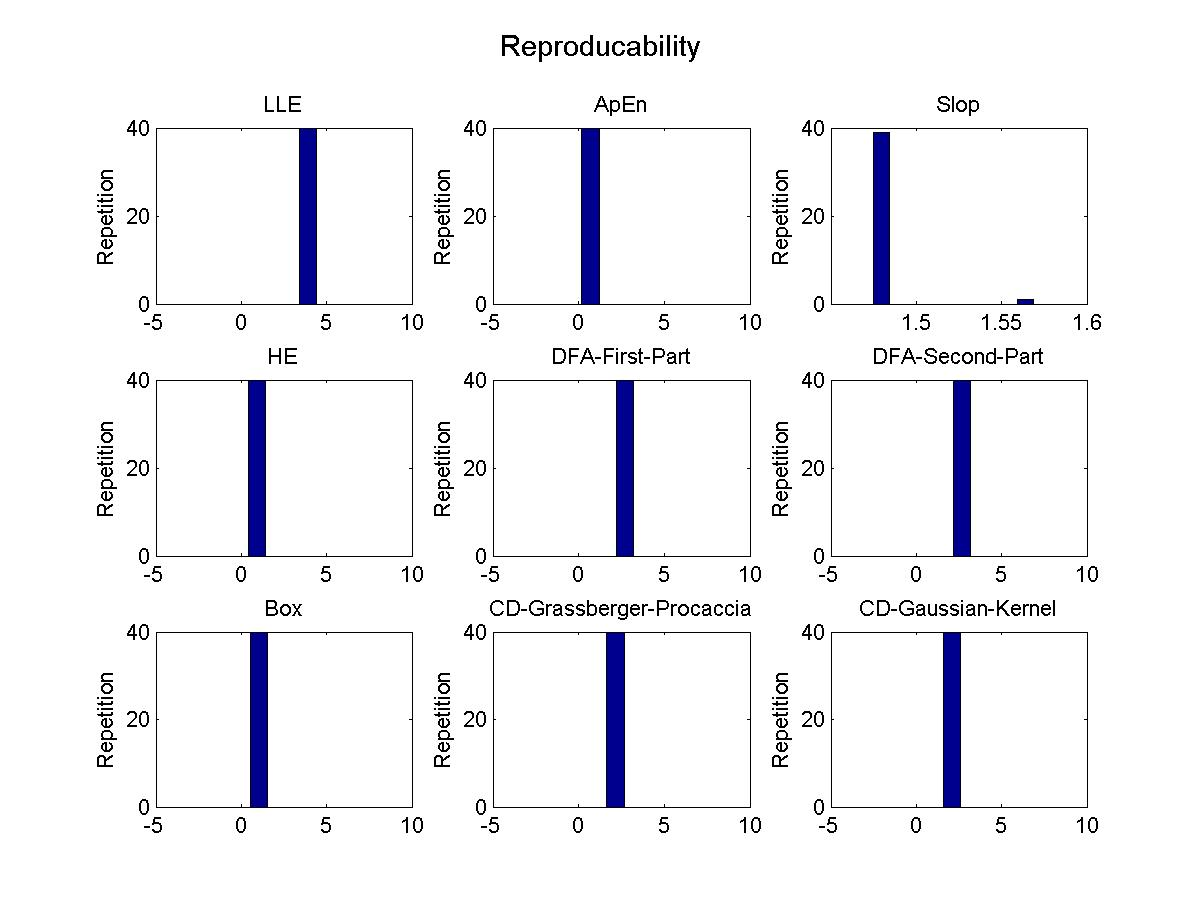
\includegraphics[width=1\linewidth]{Optional2.jpg}
\subcaption{Repeatability}\label{aaaa}
\endminipage\hfill
\minipage{0.5\textwidth}%
\centering
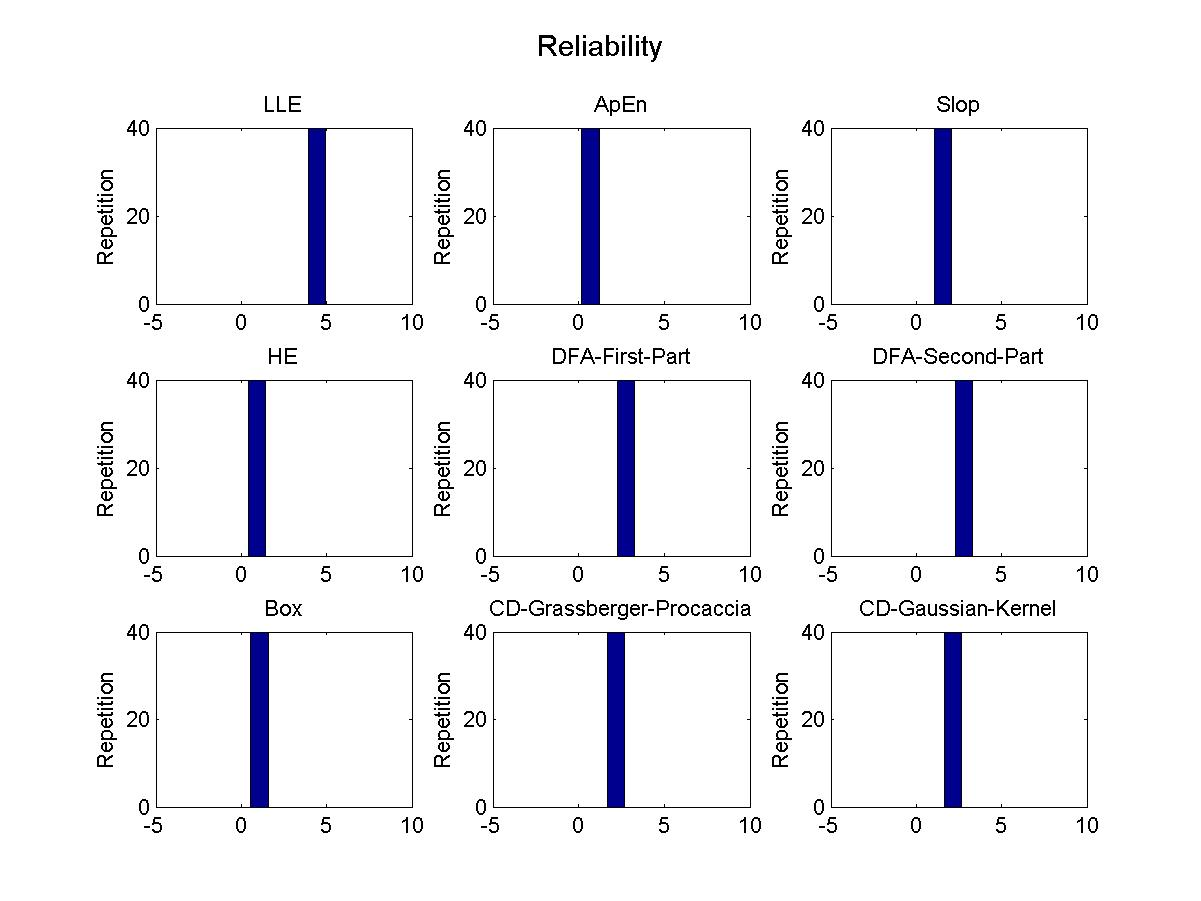
\includegraphics[width=1\linewidth]{Optional3.jpg}
\subcaption{Reliability}\label{bbbb}
\endminipage\hfill
\caption{Testing of nonlinear methods}
\end{figure}

\subsection{Discussion}

In this study the most important findings are, the ability of the nonlinear methods to estimate the chaotic behaviour of the heart rate and the possibility of getting a fully automated framework for a set of nonlinear parameter estimation. The scaling behaviour together with the fractal dimension are both capable to predict any worsening of the health patients at high duration of the ECG signals. Apart from visual inspection of the ECG measurement these approaches confirm the importance of this modality by extending utilization in different other modalities such as EEG. Patients with West syndrome reveal an breakdown of their correlation of fractals in long range measurements. All this estimation could be utilized in assessing risk of different HRV measurement in clinical bases in the near future. The disclosure of the HR dynamics in the west syndrome case is of highly importance in multimodal signal processing since in this specific case it estimate the scale of interference of the epilepsy in the heart functionality.